\begin{figure}
  \centering
  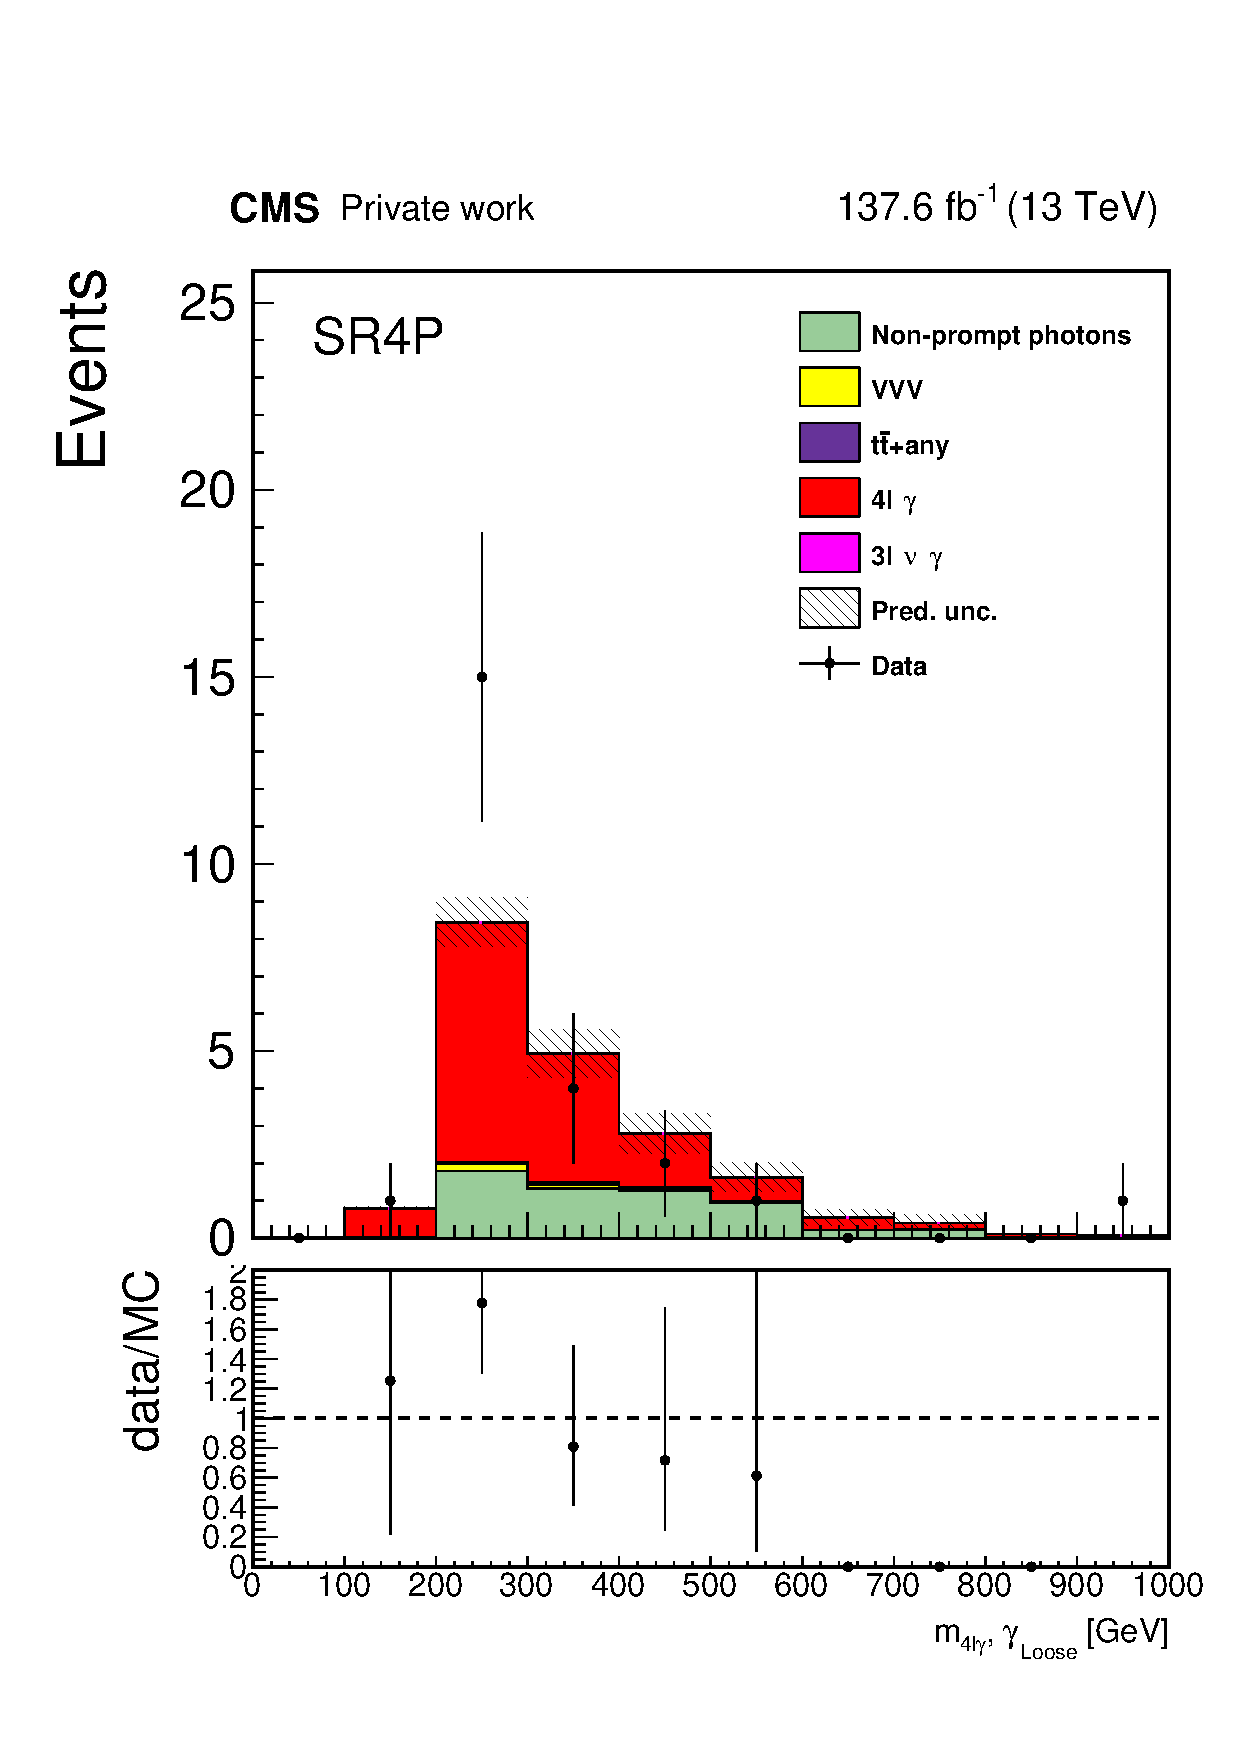
\includegraphics[height=.33\textheight]{Figures/dataMC_FSRcut/Run2/phoCR/SR4P/SYS_mZZGloose_central_pow.pdf}
  \hfill
  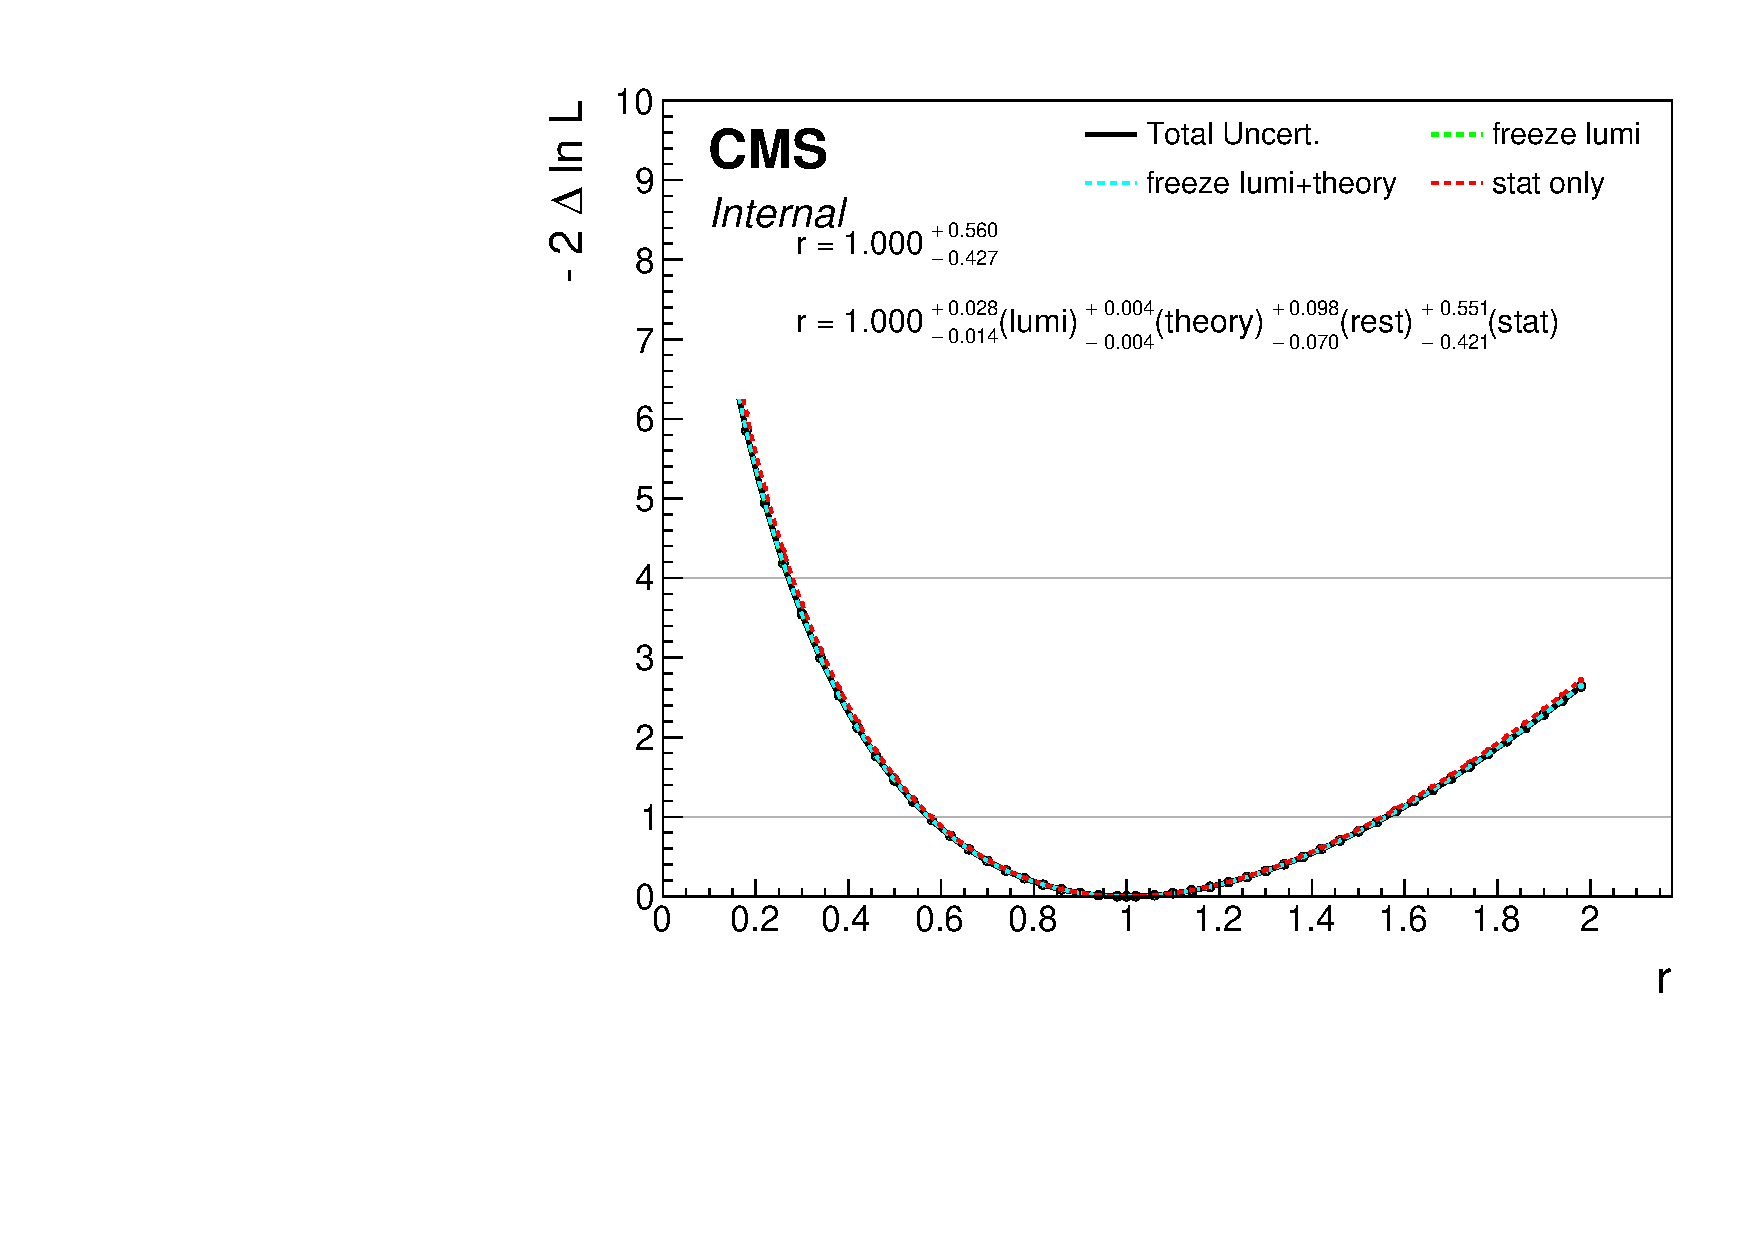
\includegraphics[height=.33\textheight]{Figures/combine/noPixVeto-mZ81/scan_expected_Run2_SR4P_phoCR_lepCR_mZZGloose.pdf}
  \caption{\captionScan{mass of the $\PZ\PZ\PGg$ system}{Loose}{cut-based ID}{d}{}}
  \label{fig:scan_FSRcut_Run2_SR4P_phoCR_lepCR_mZZGloose}
\end{figure}

\begin{figure}
  \centering
  \includegraphics[height=.33\textheight]{Figures/dataMC_FSRcut/Run2/lepCR/SR4P/SYS_loosept_central_pow.pdf}
  \hfill
  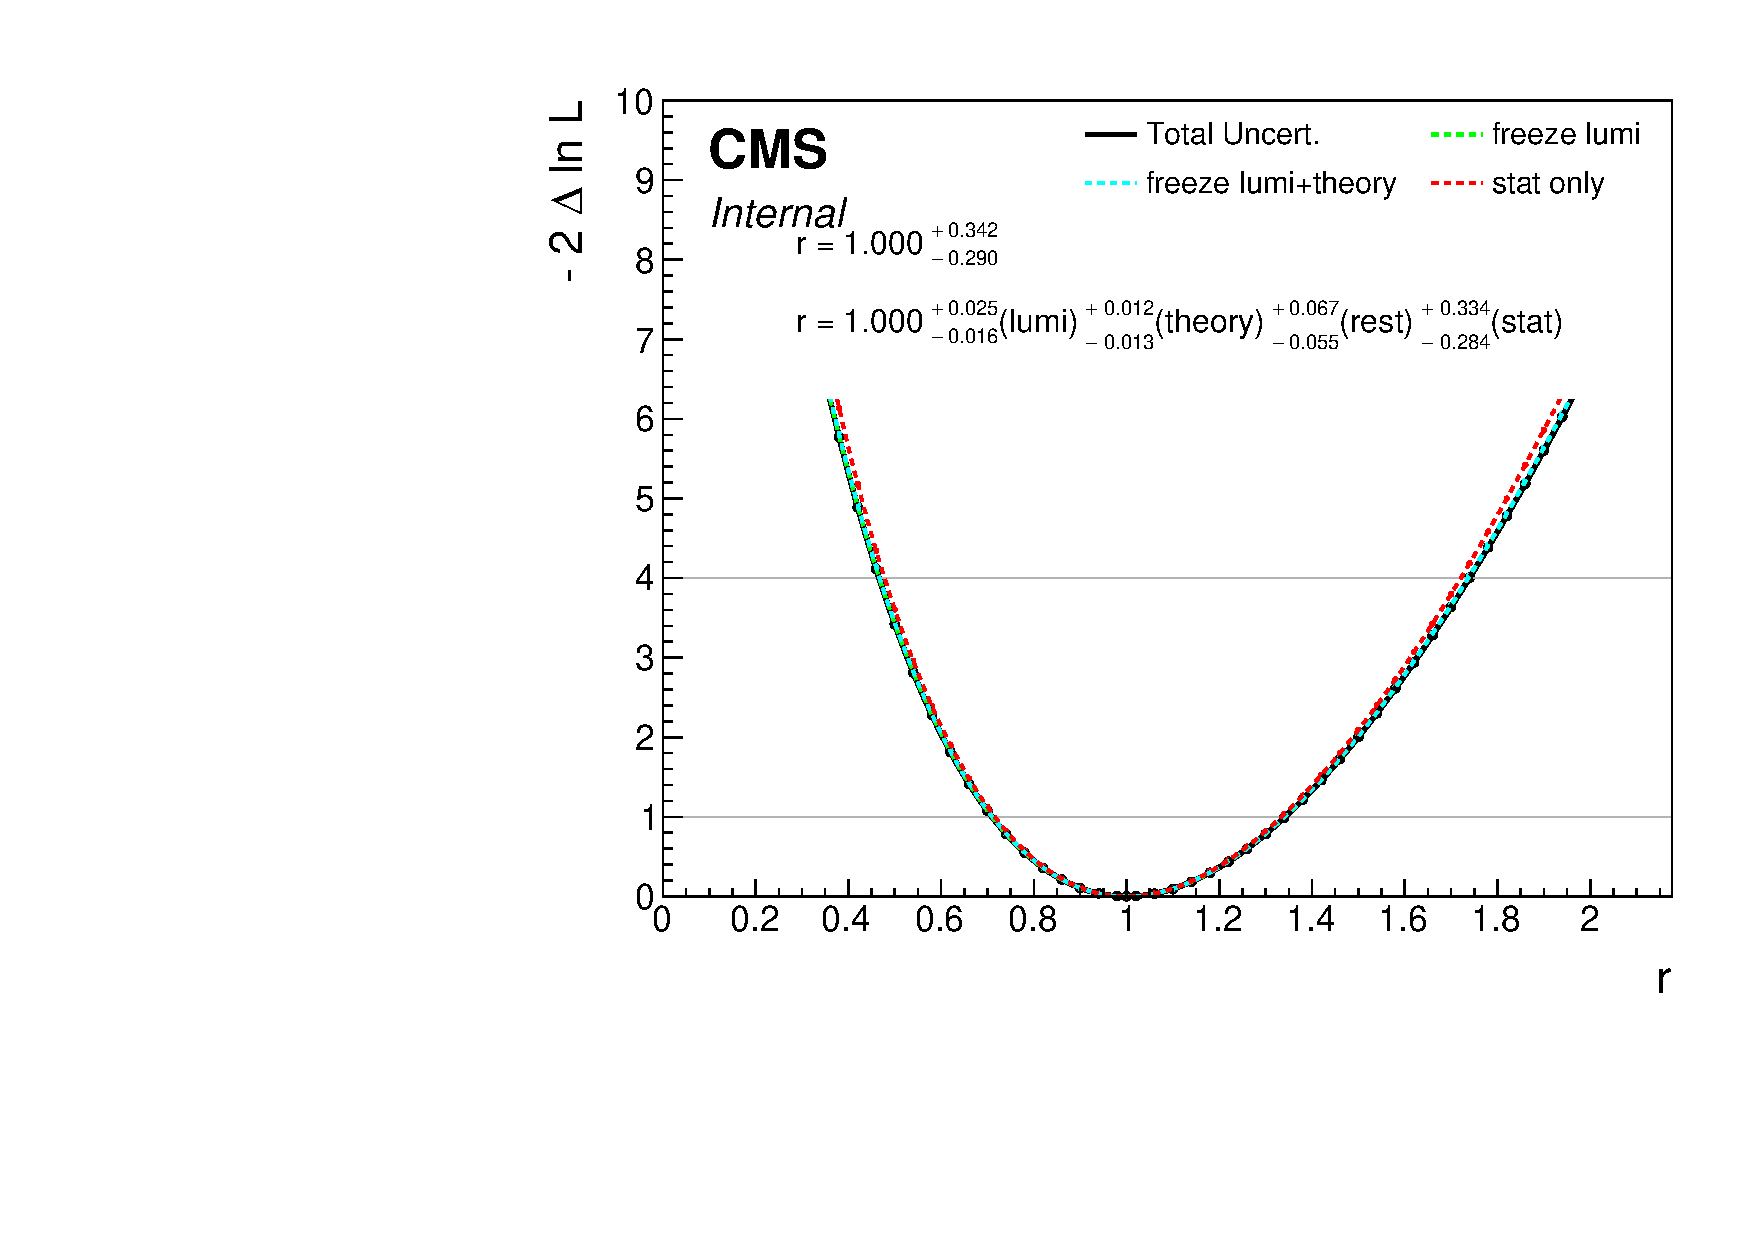
\includegraphics[height=.33\textheight]{Figures/combine/noPixVeto-mZ81/scan_expected_Run2_SR4P_phoMC_lepCR_mZZGloose.pdf}
  \caption{\captionScan{mass of the $\PZ\PZ\PGg$ system}{Loose}{cut-based ID}{s}{}}
  \label{fig:scan_FSRcut_Run2_SR4P_phoMC_lepCR_mZZGloose}
\end{figure}

\begin{figure}
  \centering
  \includegraphics[height=0.33\textheight]{Figures/dataMC_FSRcut/Run2/lepCR/SR4P/SYS_mZZGwp90_central_pow.pdf}
  \hfill
  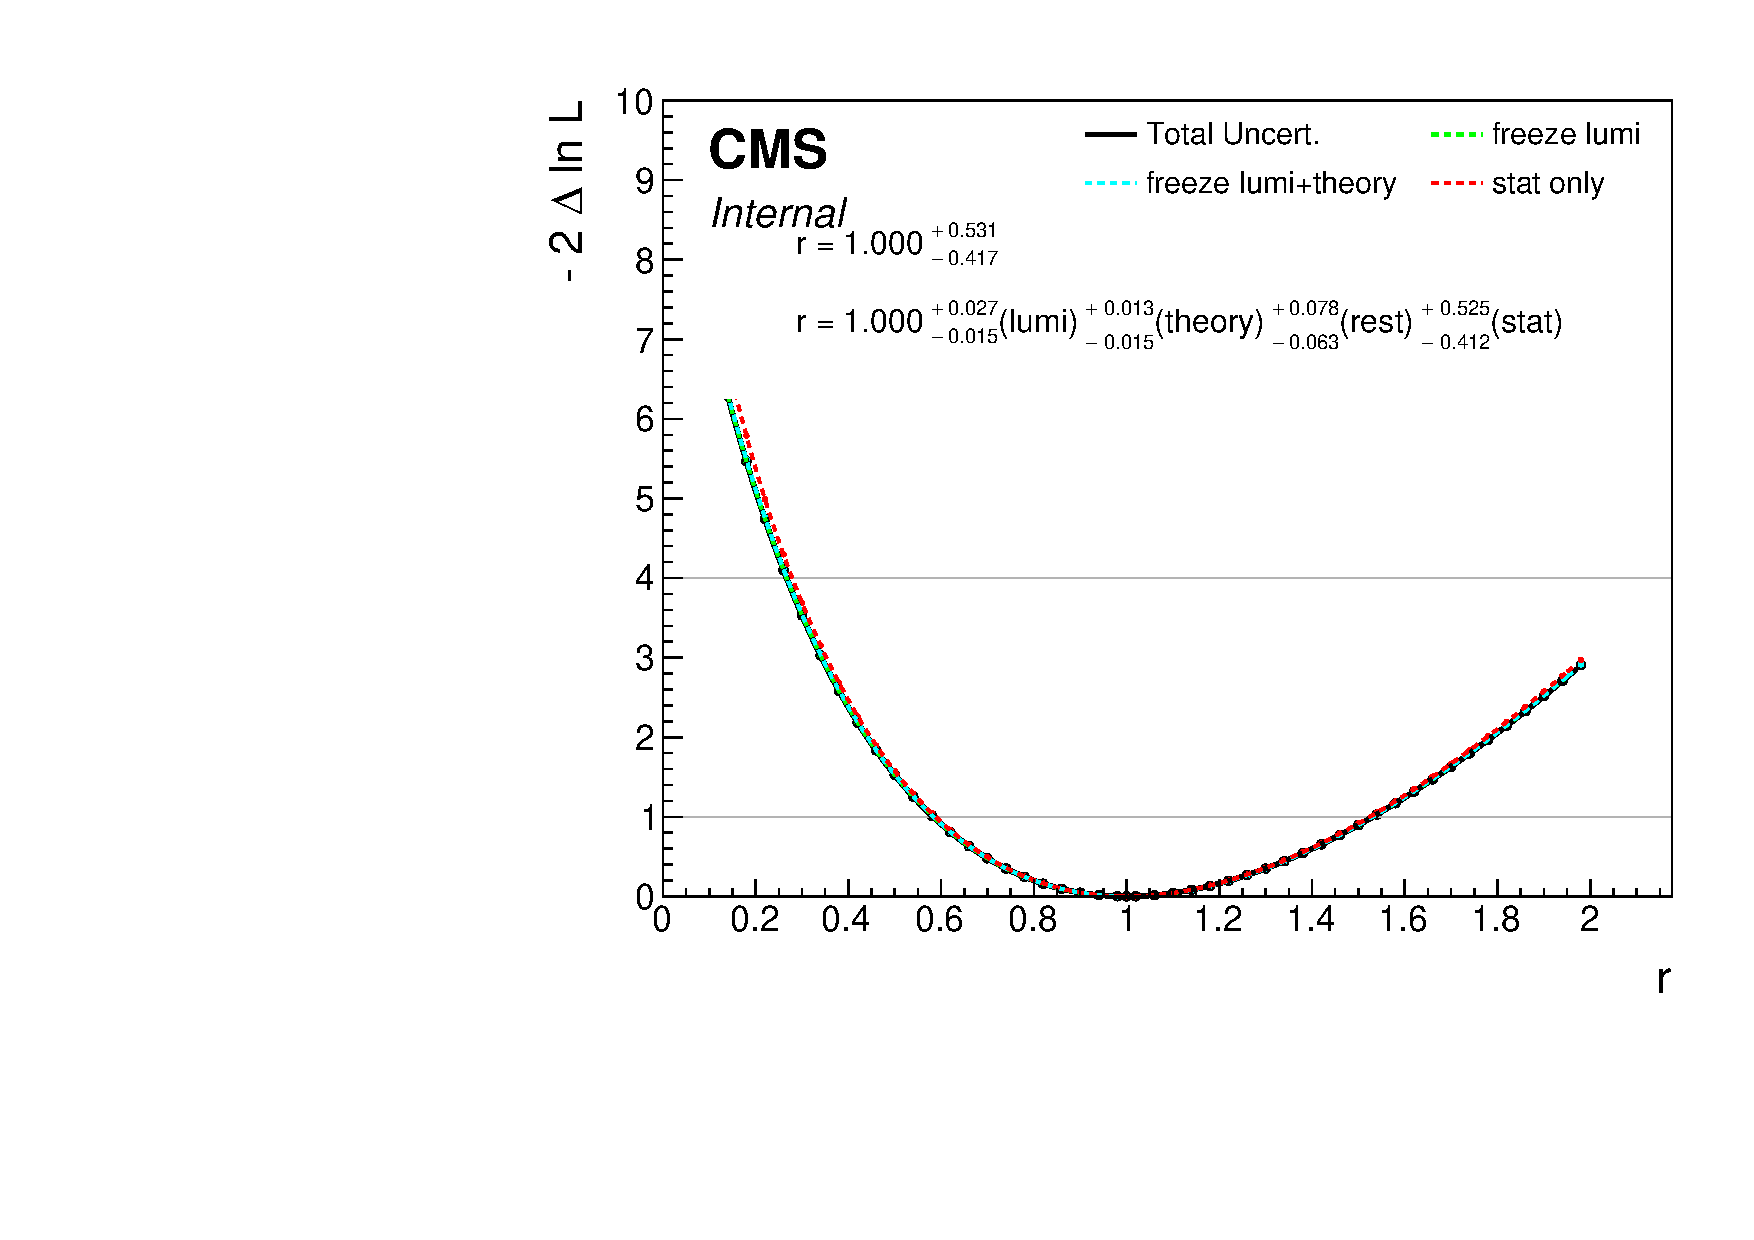
\includegraphics[height=.33\textheight]{Figures/combine/noPixVeto-mZ81/scan_expected_Run2_SR4P_phoMC_lepCR_mZZGwp90.pdf}
  \caption{\captionScan{mass of the $\PZ\PZ\PGg$ system}{\texttt{wp90}}{MVA ID}{s}{}}
  \label{fig:scan_FSRcut_Run2_SR4P_phoMC_lepCR_mZZGwp90}
\end{figure}

\begin{figure}
  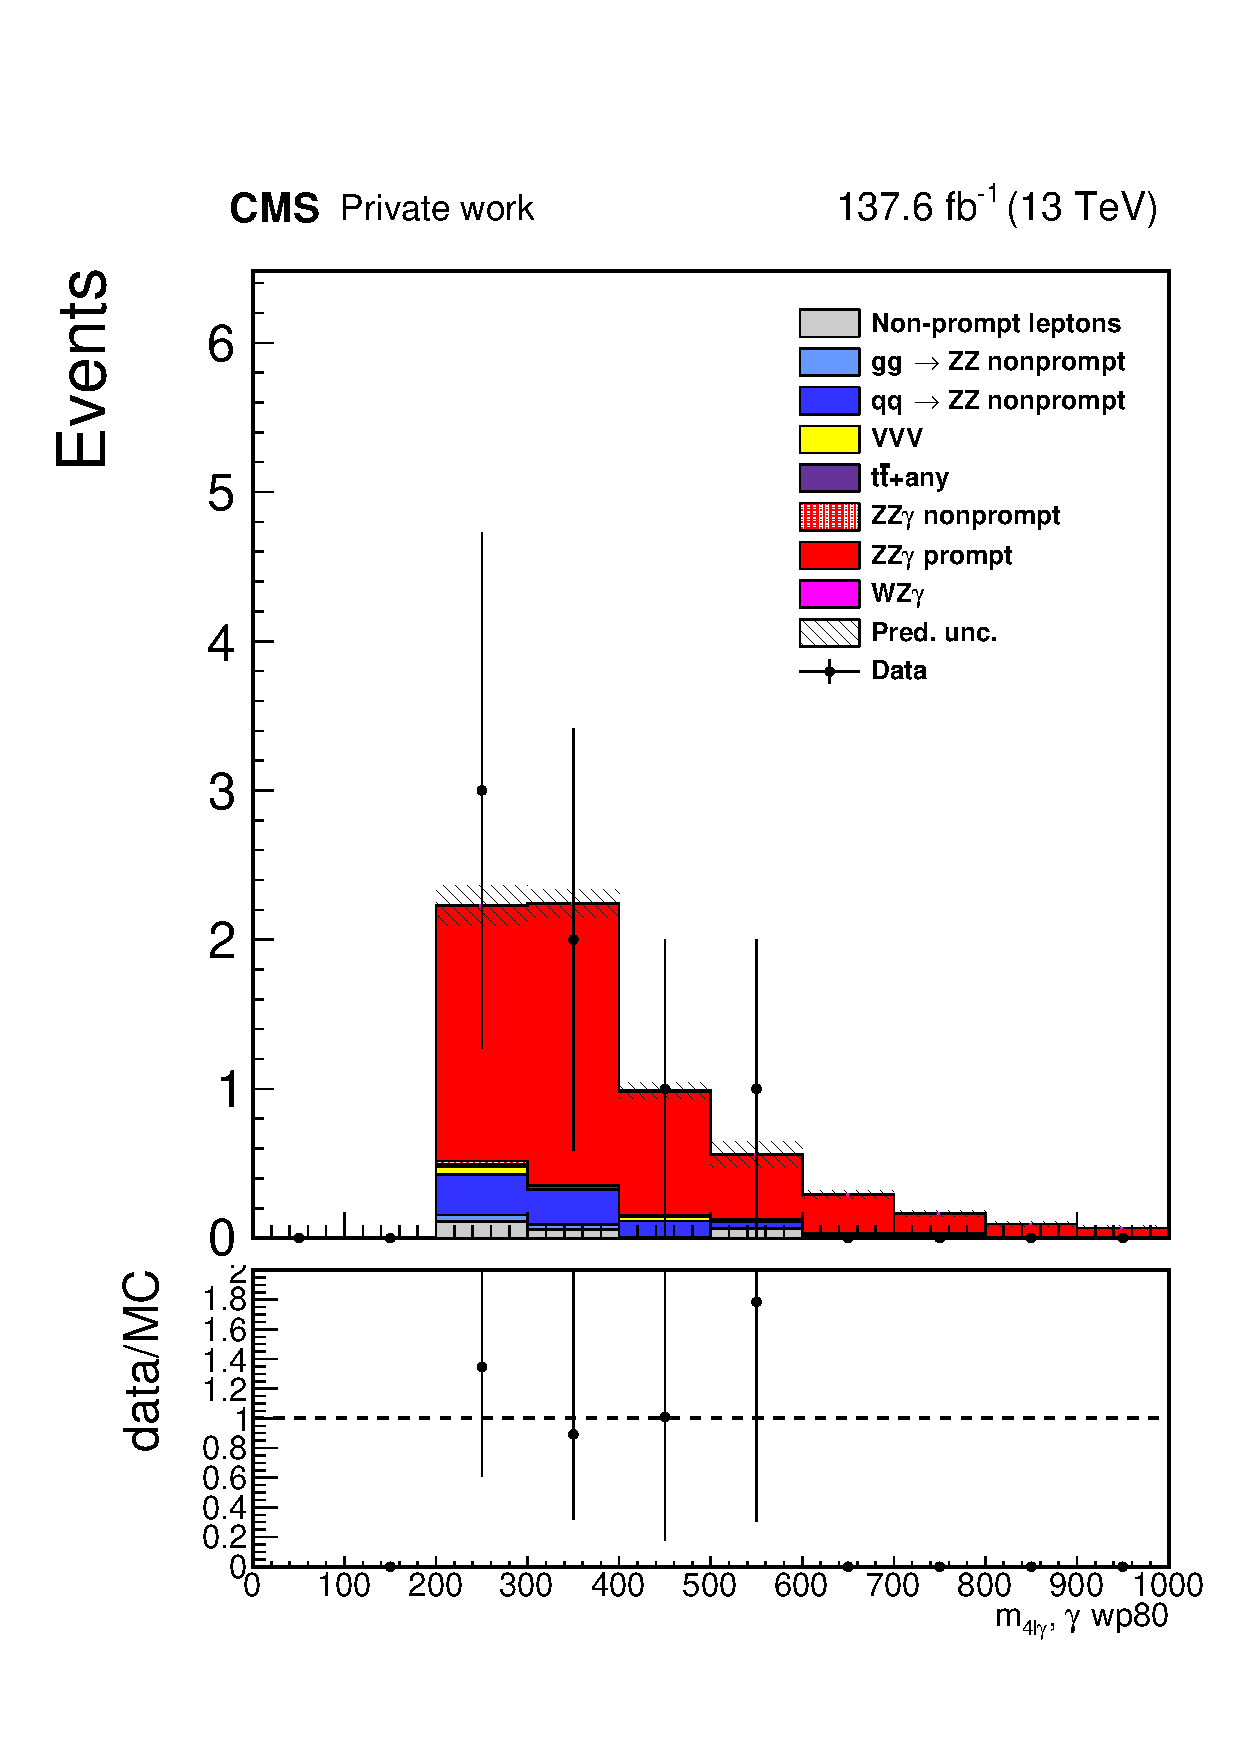
\includegraphics[height=0.33\textheight]{Figures/dataMC_FSRcut/Run2/lepCR/SR4P/SYS_mZZGwp80_central_pow.pdf}
  \hfill
  \centering
  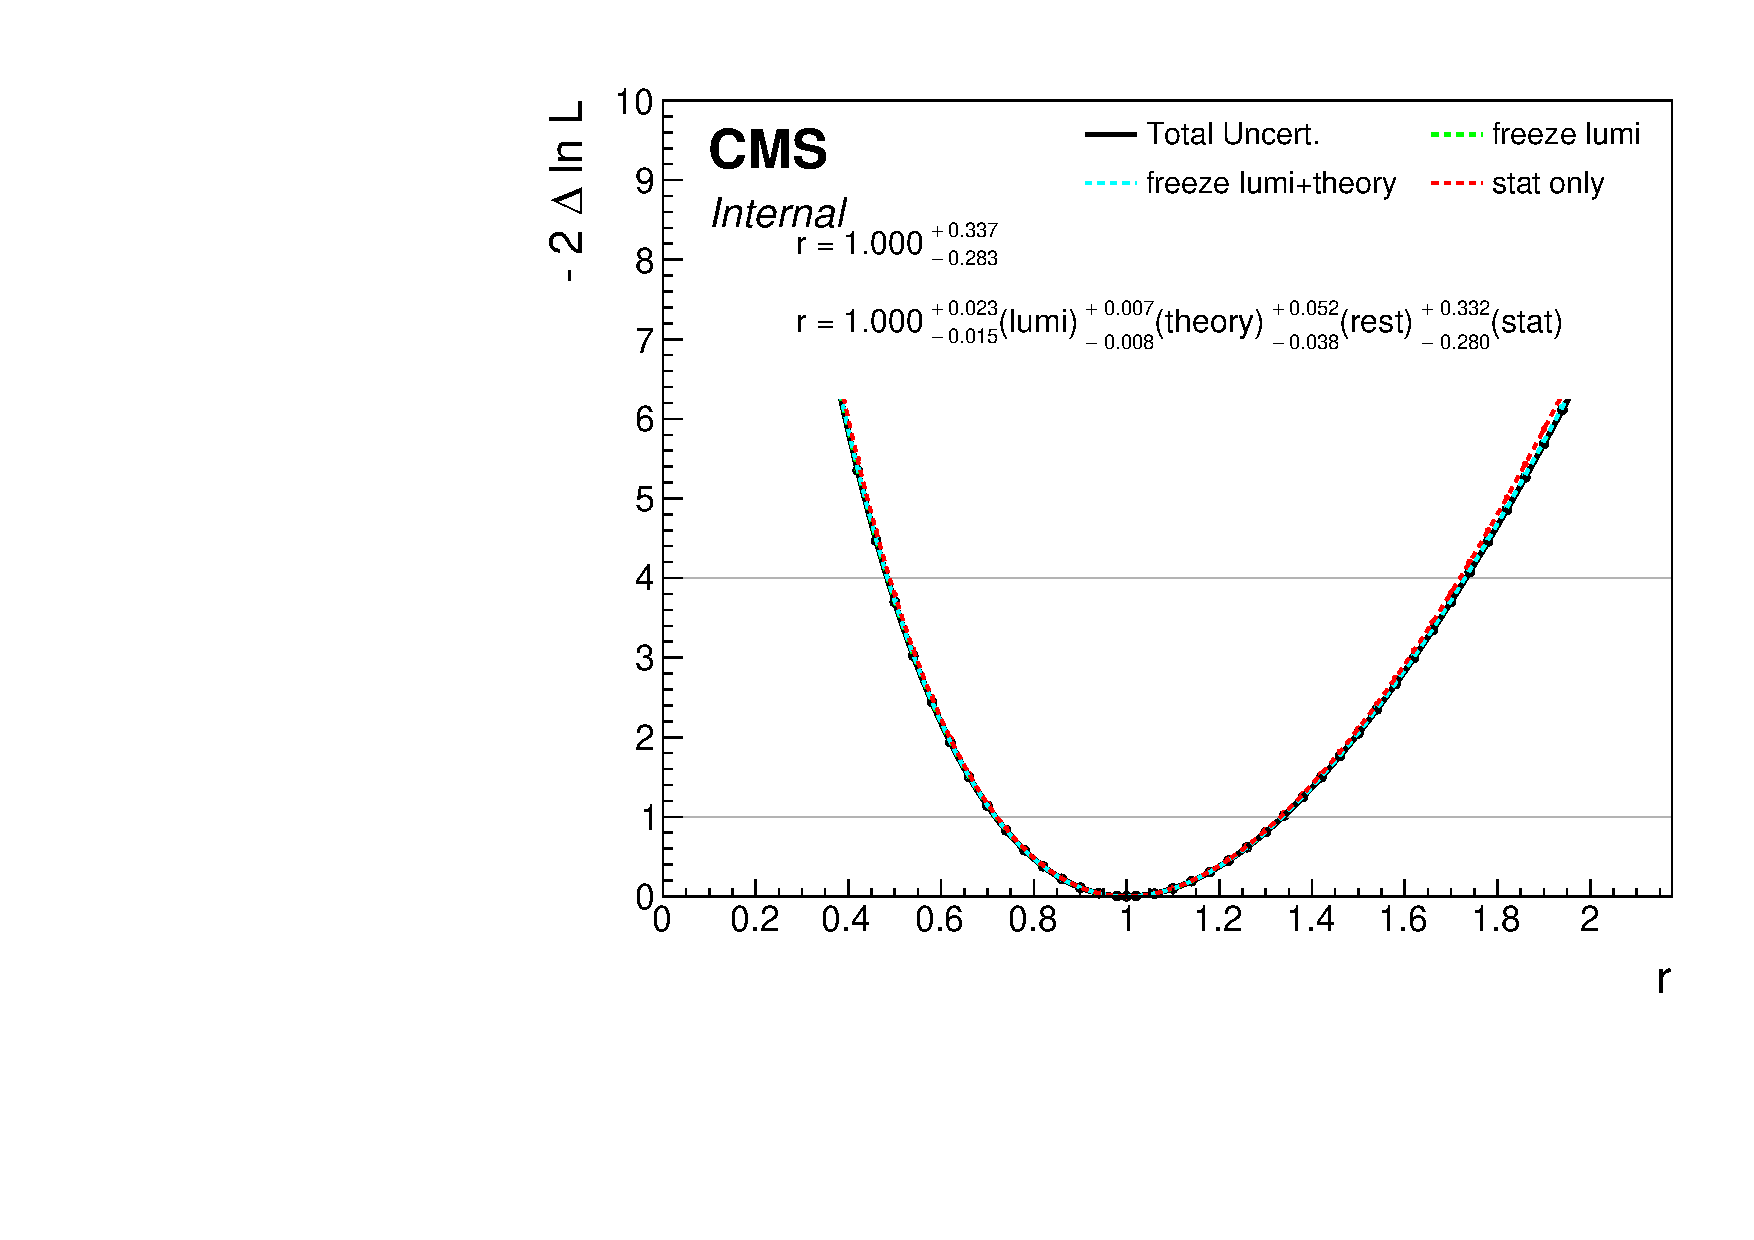
\includegraphics[height=.33\textheight]{Figures/combine/noPixVeto-mZ81/scan_expected_Run2_SR4P_phoMC_lepCR_mZZGwp80.pdf}
  \caption{\captionScan{mass of the $\PZ\PZ\PGg$ system}{\texttt{wp80}}{MVA ID}{s}{}}
  \label{fig:scan_FSRcut_Run2_SR4P_phoMC_lepCR_mZZGwp80}
\end{figure}

\begin{figure}
  \centering
  \includegraphics[height=.33\textheight]{Figures/dataMC_FSRcut/Run2/lepCR/SR4P/SYS_wp90pt_central_pow.pdf}
  \hfill
  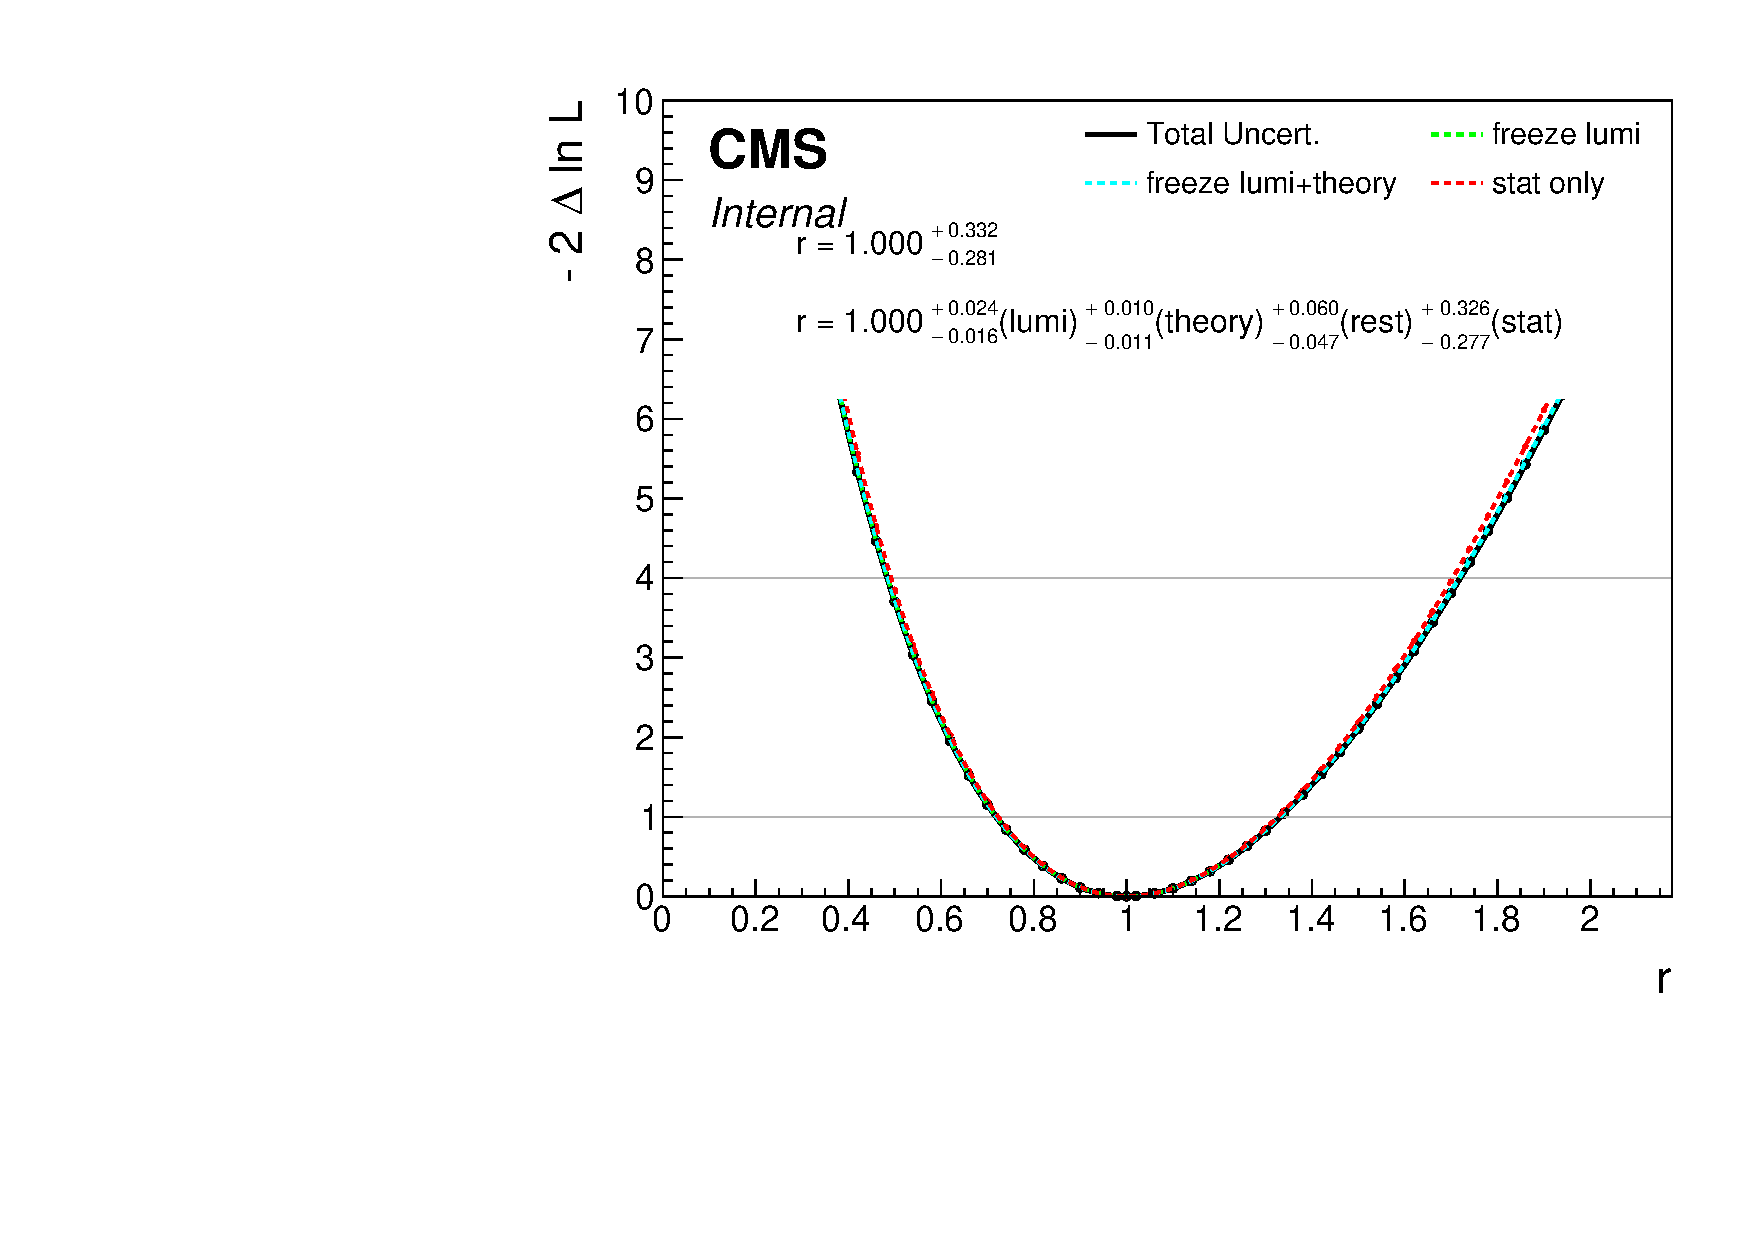
\includegraphics[height=.33\textheight]{Figures/combine/noPixVeto-mZ81/scan_expected_Run2_SR4P_phoMC_lepCR_wp90pt.pdf}
  \caption{\captionScan{transverse momentum of the photon}{\texttt{wp90}}{MVA ID}{s}{}}
  \label{fig:scan_FSRcut_Run2_SR4P_phoMC_lepCR_wp90pt}
\end{figure}

\begin{figure}
  \centering
  \includegraphics[height=.33\textheight]{Figures/dataMC_FSRcut/Run2/lepCR/SR4P/SYS_MVAcut_central_pow.pdf}
  \hfill
  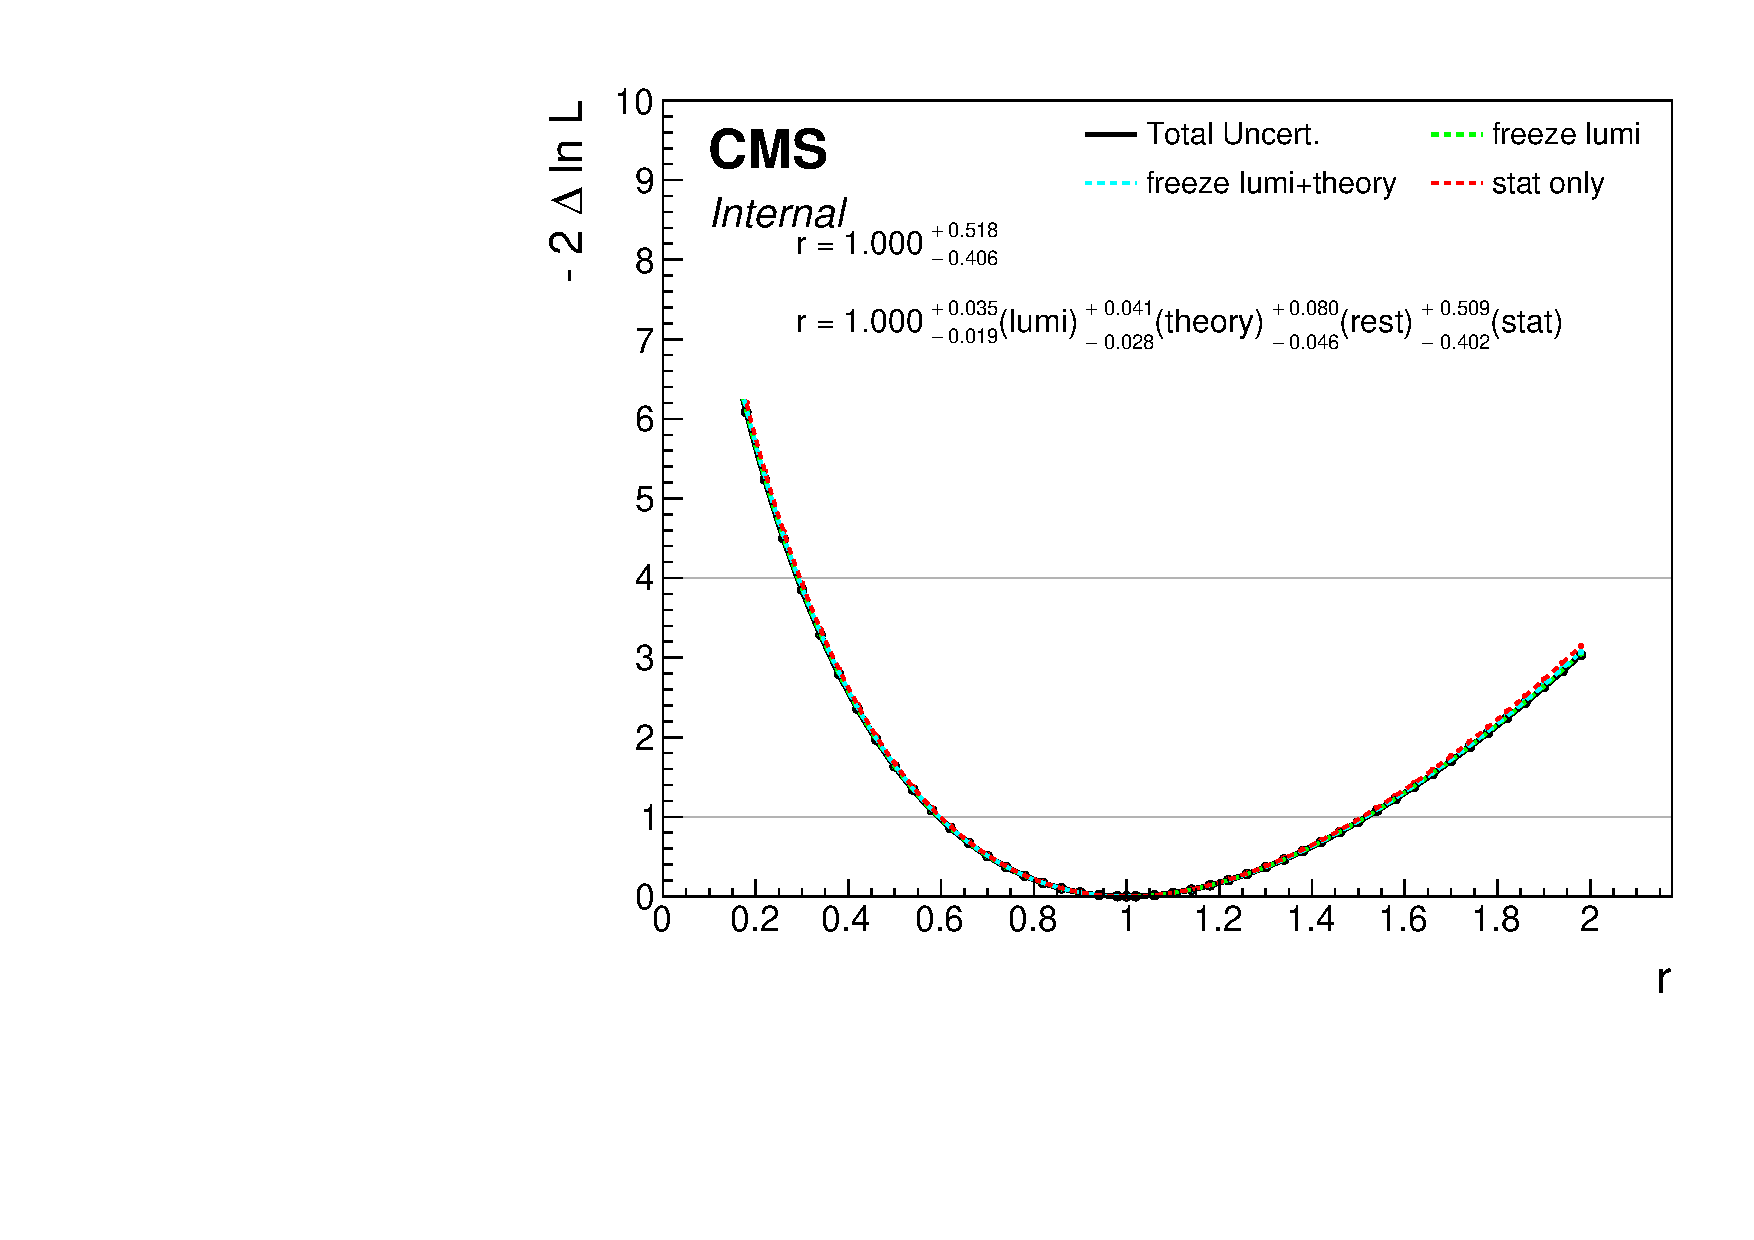
\includegraphics[height=.33\textheight]{Figures/combine/noPixVeto-mZ81/scan_expected_Run2_SR4P_phoMC_lepCR_MVAcut.pdf}
  \caption{Likelihood scan for the signal strength parameter
    on the yield in the various bins of the photon MVA ID.
    \descriptionFakePhoton{s}.
    The FSR cut is applied.
    The effect of groups of nuisance parameters on the uncertainty is assessed by sequentially fixing their value in the fit.
  }
  \label{fig:scan_FSRcut_Run2_SR4P_phoMC_lepCR_MVAcut}
\end{figure}
